% Options for packages loaded elsewhere
\PassOptionsToPackage{unicode}{hyperref}
\PassOptionsToPackage{hyphens}{url}
\PassOptionsToPackage{dvipsnames,svgnames,x11names}{xcolor}
%
\documentclass[
  letterpaper,
  DIV=11,
  numbers=noendperiod]{scrartcl}

\usepackage{amsmath,amssymb}
\usepackage{lmodern}
\usepackage{iftex}
\ifPDFTeX
  \usepackage[T1]{fontenc}
  \usepackage[utf8]{inputenc}
  \usepackage{textcomp} % provide euro and other symbols
\else % if luatex or xetex
  \usepackage{unicode-math}
  \defaultfontfeatures{Scale=MatchLowercase}
  \defaultfontfeatures[\rmfamily]{Ligatures=TeX,Scale=1}
\fi
% Use upquote if available, for straight quotes in verbatim environments
\IfFileExists{upquote.sty}{\usepackage{upquote}}{}
\IfFileExists{microtype.sty}{% use microtype if available
  \usepackage[]{microtype}
  \UseMicrotypeSet[protrusion]{basicmath} % disable protrusion for tt fonts
}{}
\makeatletter
\@ifundefined{KOMAClassName}{% if non-KOMA class
  \IfFileExists{parskip.sty}{%
    \usepackage{parskip}
  }{% else
    \setlength{\parindent}{0pt}
    \setlength{\parskip}{6pt plus 2pt minus 1pt}}
}{% if KOMA class
  \KOMAoptions{parskip=half}}
\makeatother
\usepackage{xcolor}
\setlength{\emergencystretch}{3em} % prevent overfull lines
\setcounter{secnumdepth}{5}
% Make \paragraph and \subparagraph free-standing
\ifx\paragraph\undefined\else
  \let\oldparagraph\paragraph
  \renewcommand{\paragraph}[1]{\oldparagraph{#1}\mbox{}}
\fi
\ifx\subparagraph\undefined\else
  \let\oldsubparagraph\subparagraph
  \renewcommand{\subparagraph}[1]{\oldsubparagraph{#1}\mbox{}}
\fi


\providecommand{\tightlist}{%
  \setlength{\itemsep}{0pt}\setlength{\parskip}{0pt}}\usepackage{longtable,booktabs,array}
\usepackage{calc} % for calculating minipage widths
% Correct order of tables after \paragraph or \subparagraph
\usepackage{etoolbox}
\makeatletter
\patchcmd\longtable{\par}{\if@noskipsec\mbox{}\fi\par}{}{}
\makeatother
% Allow footnotes in longtable head/foot
\IfFileExists{footnotehyper.sty}{\usepackage{footnotehyper}}{\usepackage{footnote}}
\makesavenoteenv{longtable}
\usepackage{graphicx}
\makeatletter
\def\maxwidth{\ifdim\Gin@nat@width>\linewidth\linewidth\else\Gin@nat@width\fi}
\def\maxheight{\ifdim\Gin@nat@height>\textheight\textheight\else\Gin@nat@height\fi}
\makeatother
% Scale images if necessary, so that they will not overflow the page
% margins by default, and it is still possible to overwrite the defaults
% using explicit options in \includegraphics[width, height, ...]{}
\setkeys{Gin}{width=\maxwidth,height=\maxheight,keepaspectratio}
% Set default figure placement to htbp
\makeatletter
\def\fps@figure{htbp}
\makeatother

\KOMAoption{captions}{tableheading}
\makeatletter
\makeatother
\makeatletter
\makeatother
\makeatletter
\@ifpackageloaded{caption}{}{\usepackage{caption}}
\AtBeginDocument{%
\ifdefined\contentsname
  \renewcommand*\contentsname{Table of contents}
\else
  \newcommand\contentsname{Table of contents}
\fi
\ifdefined\listfigurename
  \renewcommand*\listfigurename{List of Figures}
\else
  \newcommand\listfigurename{List of Figures}
\fi
\ifdefined\listtablename
  \renewcommand*\listtablename{List of Tables}
\else
  \newcommand\listtablename{List of Tables}
\fi
\ifdefined\figurename
  \renewcommand*\figurename{Figure}
\else
  \newcommand\figurename{Figure}
\fi
\ifdefined\tablename
  \renewcommand*\tablename{Table}
\else
  \newcommand\tablename{Table}
\fi
}
\@ifpackageloaded{float}{}{\usepackage{float}}
\floatstyle{ruled}
\@ifundefined{c@chapter}{\newfloat{codelisting}{h}{lop}}{\newfloat{codelisting}{h}{lop}[chapter]}
\floatname{codelisting}{Listing}
\newcommand*\listoflistings{\listof{codelisting}{List of Listings}}
\makeatother
\makeatletter
\@ifpackageloaded{caption}{}{\usepackage{caption}}
\@ifpackageloaded{subcaption}{}{\usepackage{subcaption}}
\makeatother
\makeatletter
\@ifpackageloaded{tcolorbox}{}{\usepackage[many]{tcolorbox}}
\makeatother
\makeatletter
\@ifundefined{shadecolor}{\definecolor{shadecolor}{rgb}{.97, .97, .97}}
\makeatother
\makeatletter
\makeatother
\ifLuaTeX
  \usepackage{selnolig}  % disable illegal ligatures
\fi
\IfFileExists{bookmark.sty}{\usepackage{bookmark}}{\usepackage{hyperref}}
\IfFileExists{xurl.sty}{\usepackage{xurl}}{} % add URL line breaks if available
\urlstyle{same} % disable monospaced font for URLs
\hypersetup{
  pdftitle={Comparison of Toronto Number of Deaths of Shelter Residents before COVID-19 and after COVID-19},
  pdfauthor={Wen Han Zhao},
  colorlinks=true,
  linkcolor={blue},
  filecolor={Maroon},
  citecolor={Blue},
  urlcolor={Blue},
  pdfcreator={LaTeX via pandoc}}

\title{Comparison of Toronto Number of Deaths of Shelter Residents
before COVID-19 and after COVID-19}
\author{Wen Han Zhao}
\date{September 24, 2024}

\begin{document}
\maketitle
\begin{abstract}
In this report, Toronto Number of Deaths of Shelter Residents is
analyzed from January 2007 to August 2024. By comparing pre-pandemic and
post-pandemic mortality data, the research aims to identify any
significant trend and changes in the health outcomes of this vulnerable
population.The findings will contribute to understanding the pandemic's
effects on homeless populations and inform future public health
interventions in shelter environments.
\end{abstract}
\ifdefined\Shaded\renewenvironment{Shaded}{\begin{tcolorbox}[borderline west={3pt}{0pt}{shadecolor}, boxrule=0pt, interior hidden, frame hidden, sharp corners, breakable, enhanced]}{\end{tcolorbox}}\fi

\hypertarget{introduction}{%
\section{Introduction}\label{introduction}}

The COVID-19 pandemic, which emerged in late 2019 and escalated globally
in early 2020, brought unprecedented challenges to public health
systems, economies, and vulnerable populations. As governments worldwide
imposed lockdowns and implemented social distancing measures to curb the
virus's spread, homeless populations, including shelter residents, faced
heightened risks. Overcrowded living conditions, limited access to
healthcare, and underlying health issues made shelter residents
particularly susceptible to COVID-19 infections. In Toronto, the
pandemic raised concerns about the potential for an increased number of
deaths among shelter residents, driven by both direct infection and the
pandemic's broader social and economic impacts. This study seeks to
analyze whether the number of deaths among shelter residents in Toronto
increased significantly during the pandemic compared to the pre-pandemic
period.

\hypertarget{overview}{%
\section{Overview}\label{overview}}

The ``Deaths of Shelter Residents'' dataset from Toronto Open Data
provides annual records of deaths among individuals living in Toronto's
homeless shelters. It includes data on the total number of deaths,
broken down by year, from 2007 to the most recent available data. The
dataset also categorizes deaths by gender. Additionally, it may include
monthly data, allowing for a more granular analysis of trends over time.
This dataset is useful for tracking mortality patterns among shelter
residents and identifying any significant changes, such as an increase
in deaths during the COVID-19 pandemic.

\hypertarget{data}{%
\section{Data}\label{data}}

After loading the dataset using the R programming language (R Core Team
2022) and the here package (Müller 2020), the tidyverse (Wickham et
al.~2019) package was used to generate graphs. In doing so, R code was
adapted from Alexander (2024).

\begin{verbatim}
`geom_smooth()` using method = 'loess' and formula = 'y ~ x'
\end{verbatim}

\begin{figure}

{\centering 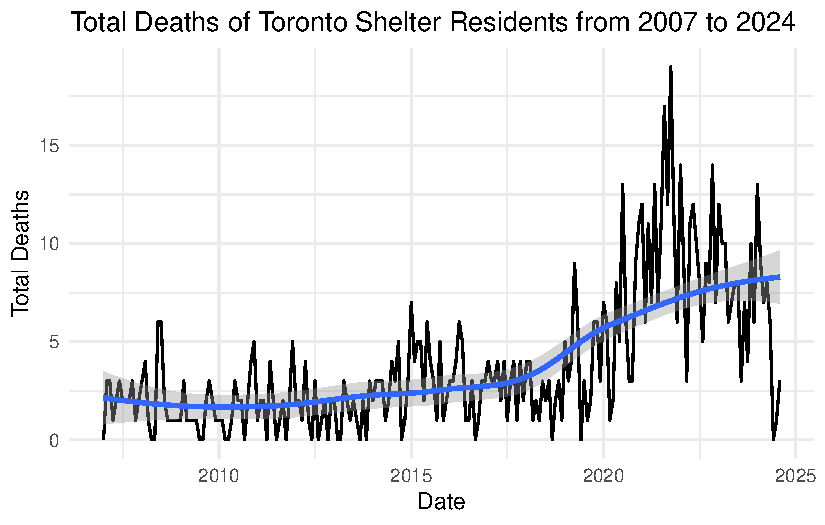
\includegraphics{paper_files/figure-pdf/fig-deaths-1.pdf}

}

\caption{\label{fig-deaths}Deaths of shelter residents over time}

\end{figure}

The graph illustrates the total number of deaths among Toronto shelter
residents from 2007 to 2024, showing an increasing trend over time. Key
observations include:

Early Years (2007--2015): The number of deaths fluctuated relatively
mildly, generally remaining below five deaths per reporting period, with
some sporadic spikes.

2015--2020: Starting around 2015, the frequency and magnitude of death
counts began to rise, indicating an upward trend. The gradual increase
suggests that factors affecting shelter residents' health, such as
access to care or living conditions, may have started to worsen even
before the pandemic.

COVID-19 Period (2020 onwards): The most notable trend is the sharp
increase in deaths from 2020 onwards, which corresponds with the
COVID-19 pandemic. The number of deaths spikes significantly during this
period, reaching highs of 10--15 deaths in some months, suggesting a
strong impact of the pandemic on shelter residents.

Post-2022: Following the pandemic's peak, death numbers show a more
volatile pattern, but the overall trend remains elevated compared to the
pre-pandemic years, with a generally higher baseline.

The trendline (blue line) further confirms the long-term upward
trajectory, with an acceleration in death counts from 2020, likely
driven by pandemic-related factors such as increased health risks,
inadequate shelter conditions, or reduced access to healthcare during
the pandemic. The shading around the line shows the confidence interval,
which suggests that the pattern observed is statistically significant.

This graphical analysis highlights a considerable increase in deaths
among shelter residents during and following the COVID-19 pandemic,
aligning with the hypothesis that the pandemic significantly impacted
mortality in this population. Total Deaths of Toronto Male Shlter
Residents from 2007 to 2024.

\begin{verbatim}
`geom_smooth()` using method = 'loess' and formula = 'y ~ x'
\end{verbatim}

\begin{figure}

{\centering 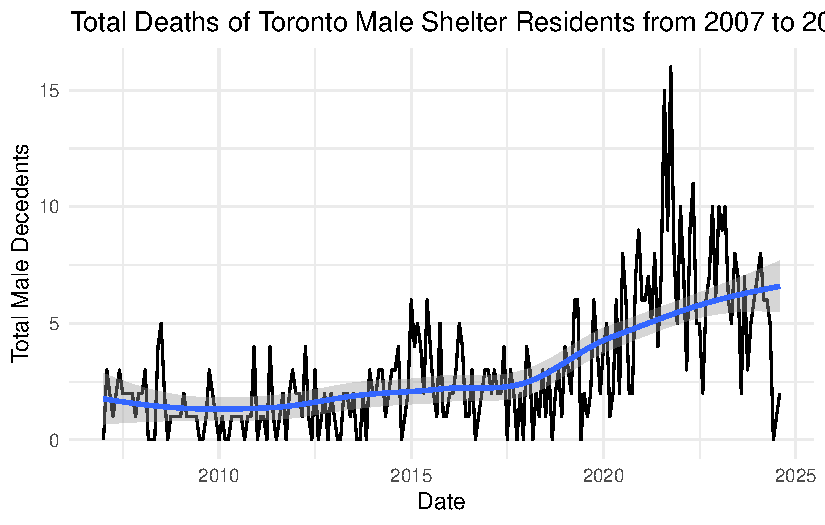
\includegraphics{paper_files/figure-pdf/fig-male_decedents-1.pdf}

}

\caption{\label{fig-male_decedents}Deaths of male shelter residents over
time}

\end{figure}

The graph illustrates the total number of deaths among Toronto male
shelter residents from 2007 to 2024, showing an increasing trend over
time. Key observations include:

The overall graph has similar pattern to the total numbers of deaths and
it has spiked significantly in 2022. We could also spot a recurring
trend in some of the months of a year, which could be interesting to
analysis.

The trendline (blue line) further confirms the long-term upward
trajectory, with an acceleration in death counts from 2020, likely
driven by pandemic-related factors such as increased health risks,
inadequate shelter conditions, or reduced access to healthcare during
the pandemic. The shading around the line shows the confidence interval,
which suggests that the pattern observed is statistically significant.

This graphical analysis highlights a considerable increase in deaths
among shelter residents during and following the COVID-19 pandemic,
aligning with the hypothesis that the pandemic significantly impacted
mortality in this population. Total Deaths of Toronto Male Shlter
Residents from 2007 to 2024.

\begin{verbatim}
`geom_smooth()` using method = 'loess' and formula = 'y ~ x'
\end{verbatim}

\begin{figure}

{\centering 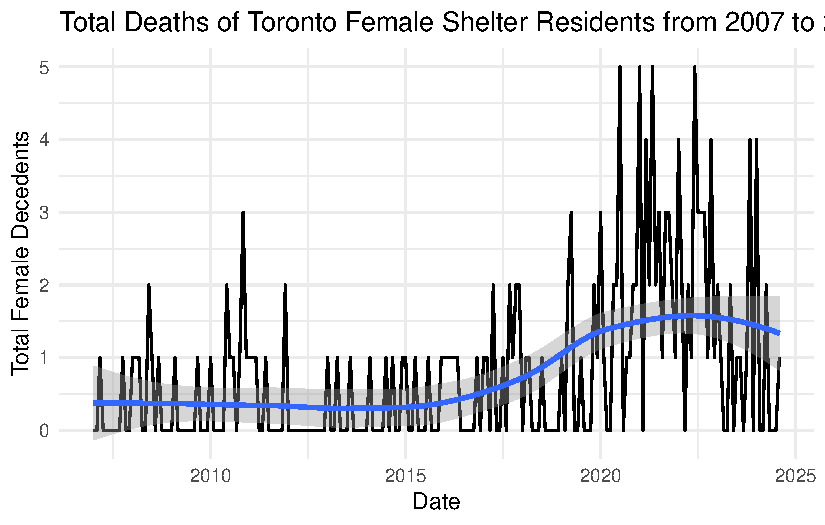
\includegraphics{paper_files/figure-pdf/fig-female_decedents-1.pdf}

}

\caption{\label{fig-female_decedents}Deaths of female shelter residents
over time}

\end{figure}

The graph illustrates the total number of deaths among Toronto female
shelter residents from 2007 to 2024, showing an increasing trend over
time. Key observations include:

The overall graph has similar pattern to the total numbers of deaths and
it has spiked significantly in 2022. Female shelter residents seems to
be greater than male compared to the last graph. This could suggest that
during COVID-19 and post COVID-19, female shelter residents have a
higher chance of death. We could also spot a recurring trend in some of
the months of a year, which could be interesting to analysis.

The trendline (blue line) further confirms the long-term upward
trajectory, with an acceleration in death counts from 2020, likely
driven by pandemic-related factors such as increased health risks,
inadequate shelter conditions, or reduced access to healthcare during
the pandemic. The shading around the line shows the confidence interval,
which suggests that the pattern observed is statistically significant.

This graphical analysis highlights a considerable increase in deaths
among shelter residents during and following the COVID-19 pandemic,
aligning with the hypothesis that the pandemic significantly impacted
mortality in this population. Total Deaths of Toronto female Shlter
Residents from 2007 to 2024.

\hypertarget{discussion}{%
\section{Discussion}\label{discussion}}

The analysis of the ``Deaths of Shelter Residents'' dataset reveals a
significant increase in mortality rates among shelter residents in
Toronto following 2020. This upward trend may reflect the compounded
effects of various factors, including the COVID-19 pandemic, which
exacerbated existing vulnerabilities such as mental health issues,
substance abuse, and access to healthcare. The pandemic's impact likely
intensified the challenges faced by homeless populations, including
increased social isolation, reduced access to support services, and
heightened risks of exposure to the virus. Additionally, systemic issues
such as housing instability, economic hardship, and inadequate social
safety nets may have contributed to this alarming rise in deaths. This
data underscores the urgent need for targeted interventions and policy
reforms to address the complex needs of this vulnerable population and
improve their overall health and well-being.

\hypertarget{weaknesses-and-next-steps}{%
\subsection{Weaknesses and next steps}\label{weaknesses-and-next-steps}}

The cause of total deaths of shelter residents is unknown, so we do not
know for sure if the deaths is caused by COVID-19 only. If we could have
a data that has the cause of deaths would give us more confidence in our
testing.

\newpage

\hypertarget{references}{%
\section{References}\label{references}}



\end{document}
